\section{Transactions}\label{transactions}

As there are no miners in the network, transactions are being validated by other nodes that issue transactions themselves. In order to create a new transaction on the network, a node does the following steps:
\begin{enumerate}
    \item The node chooses two unconfirmed transactions according to an Monte Carlo Walk algorithm which will be described in more detail in Section \ref{tip-selection}.
    \item The node is responsible for checking the validity of these two transactions. Conflicting transactions are ignored.
    \item A node has to perform a cryptographic puzzle in order to make the new transaction valid. Similar to the Proof of Work (PoW) mechanism in Bitcoin, this puzzle is solved with computational resources. The puzzle is defined by finding a nonce such that the hash of this number concatenated with some data from the approved transactions results in a number smaller than some predefined constant. This puzzle is necessary in order to prevent several attack scenarios which will be discussed in Chapter \ref{attacks}.
\end{enumerate}

The next section describes the basic concepts of the tangle. For all figures, a box resembles a transaction and the directed edge between nodes illustrates the approval of a transactions. In order to understand the approval algorithm, the following five parameters are defined for every transaction.
\begin{description}
    \item[weight] The weight of a transaction is defined by the amount of work that the issuing node has invested in to this transaction. The weight of a transaction resembles its importance. This measurement helps to prevent spamming and other attacks since no node can create an abundance of transactions with meaningful weights within a short period of time. 
    \item[cumulative weight] The cumulative weight of a transaction is calculated by the weight of the transaction itself plus the sum of all transactions that directly or indirectly approve this transaction. Figure \ref{fig:cumulative-weight} shows how the weight and the cumulative weight change after the new transaction \textit{X} is added, the smaller number denotes the weight of a node and the bold number represents cumulative weight of a transaction.\par
        \begin{minipage}{\linewidth}
            \centering
            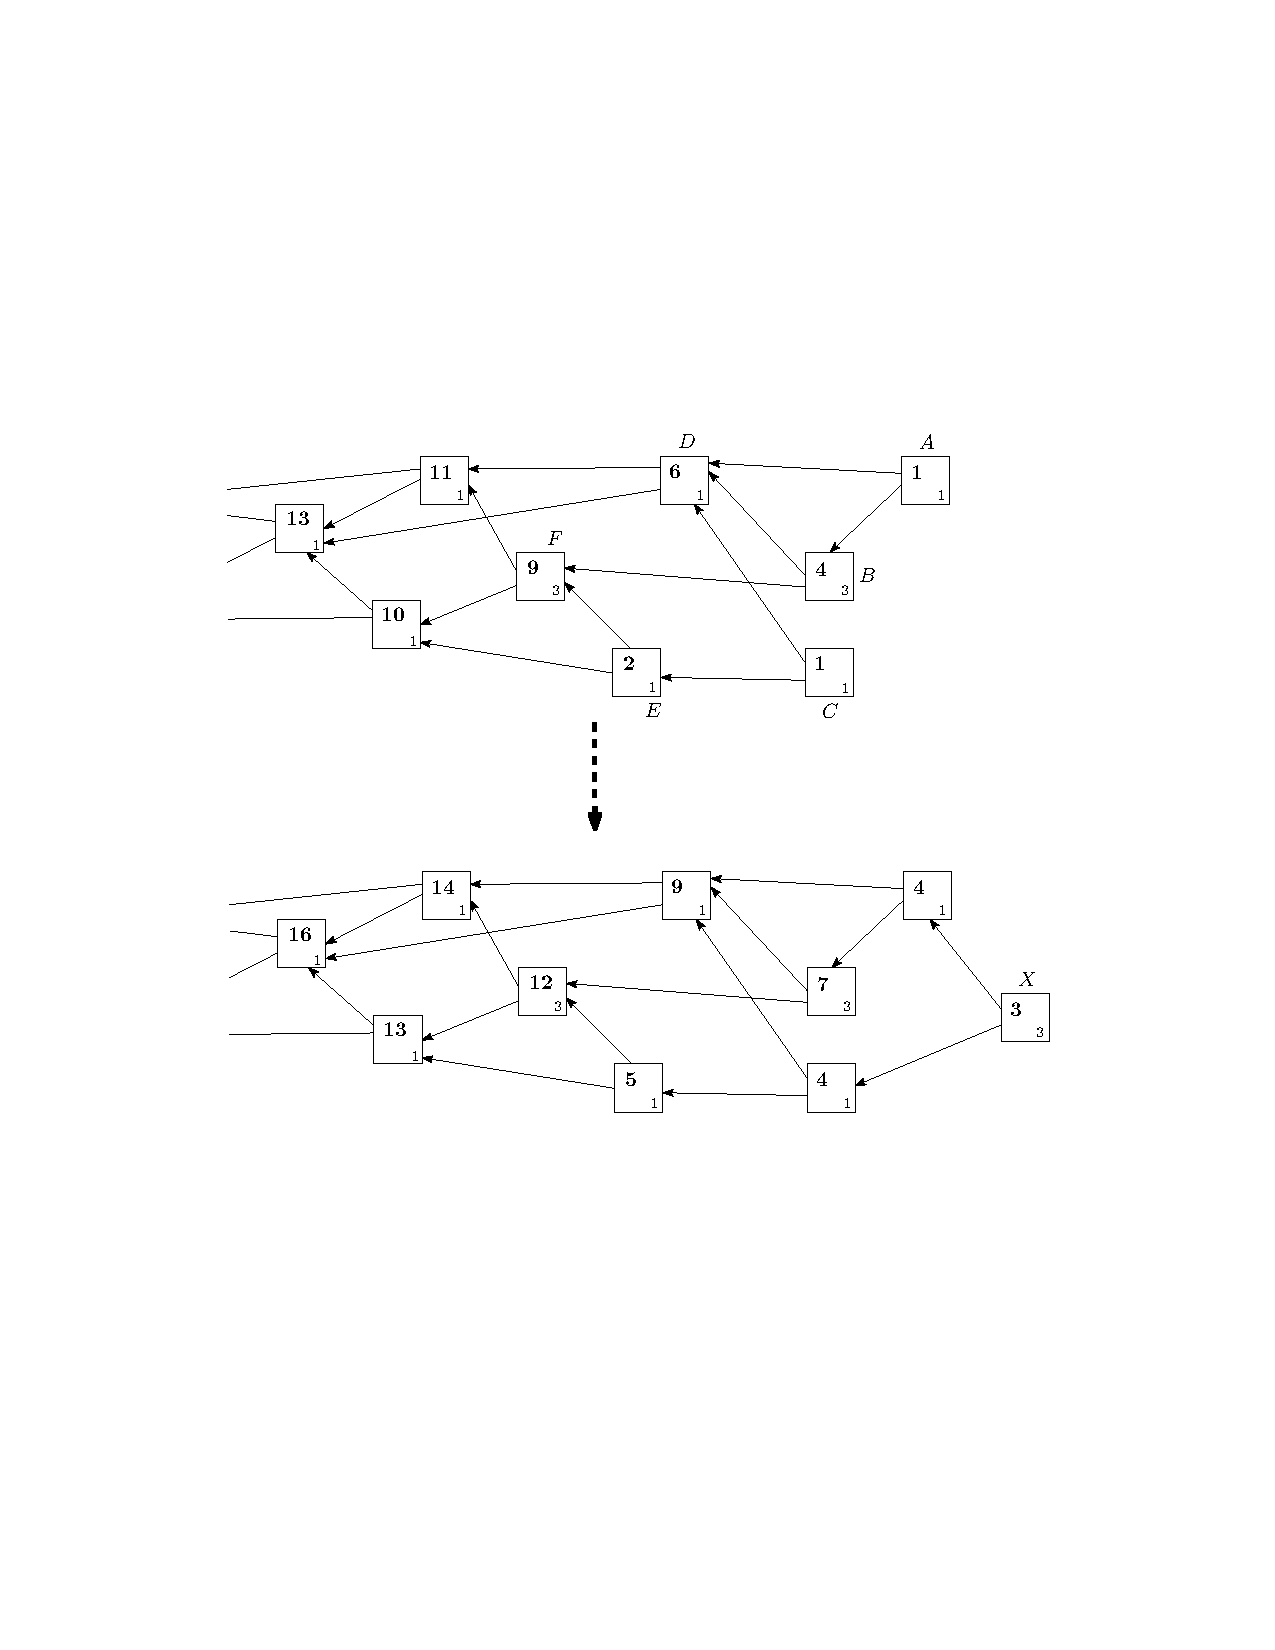
\includegraphics[width=10cm]{images/cummulative_weight.pdf}
            \captionof{figure}{Cumulative Weight \cite{the-tangle}}
            \label{fig:cumulative-weight}
        \end{minipage}
    \item[height] The height of a transaction is the length of the longest oriented path to the genesis transaction. In Figure \ref{fig:height-depth-score}, transaction \textit{G} has a height of 1 due to the blue edge.
    \item[depth] The depth of a transaction is the length of the longest reverse oriented path to some tip. In Figure \ref{fig:height-depth-score}, transaction \textit{G} has a depth of 4 due to the red approvals from newer transactions \textit{F, D, B} and \textit{A}.
    \item[score] The score of a transaction is the sum of weights of all transactions that are approved by this transaction plus its own weight. The scores for transactions \textit{A} and \textit{C} are shown with the circled number in Figure \ref{fig:height-depth-score}.\par
        \begin{minipage}{\linewidth}
            \centering
            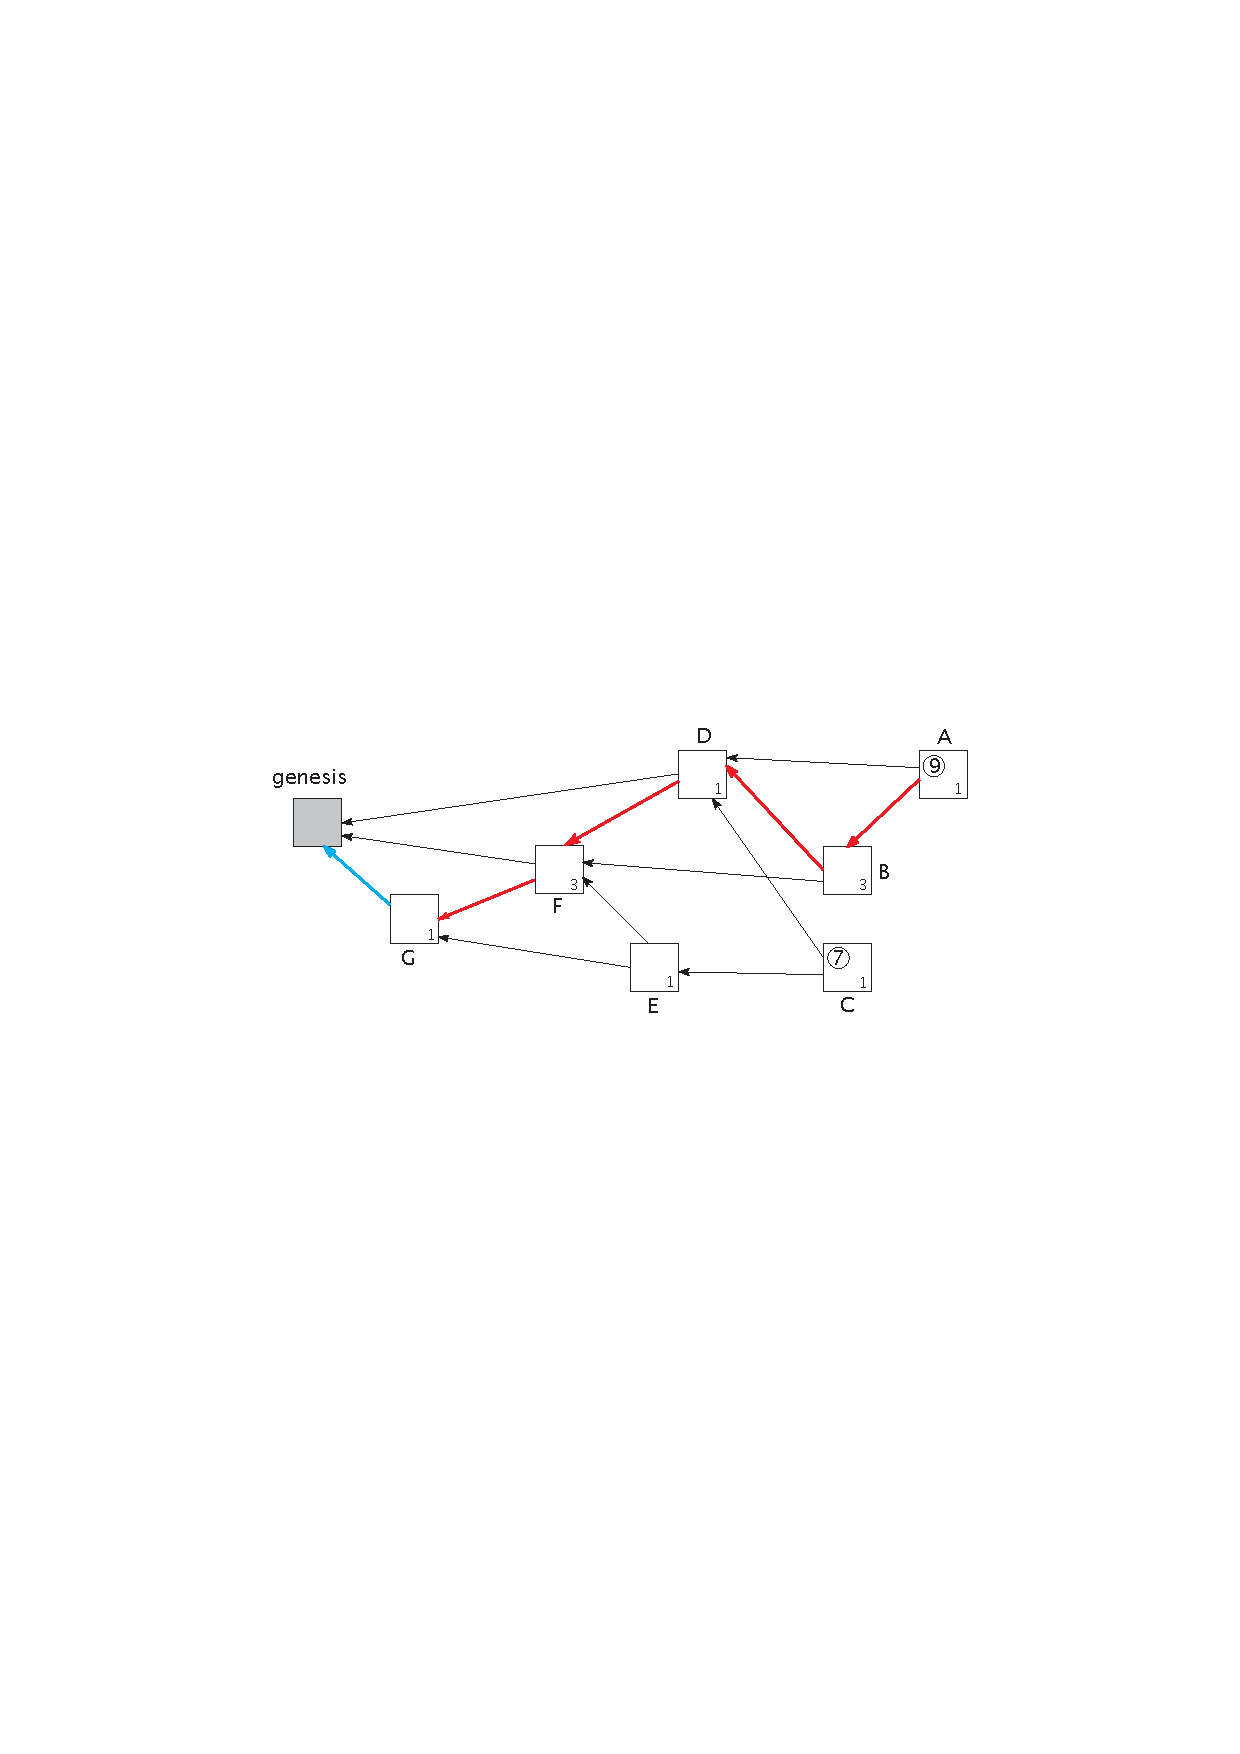
\includegraphics[width=12cm]{images/height-depth-score.pdf}
            \captionof{figure}{Height, Depth and Score \cite{the-tangle}}
            \label{fig:height-depth-score}
        \end{minipage}
\end{description}

These parameters will play an important role when discussing tip selection in Section \ref{tip-selection} and attack scenarios \ref{attacks}.